\chapter{Imágenes}
%
\section{Insertar imagen}
Para incluir imágenes se puede usar el asistente de TeXstudio cuya interfaz es la mostrada en la figura \ref{fig:auxiliar-imagenes}.

\begin{figure}[h]
	\centering
	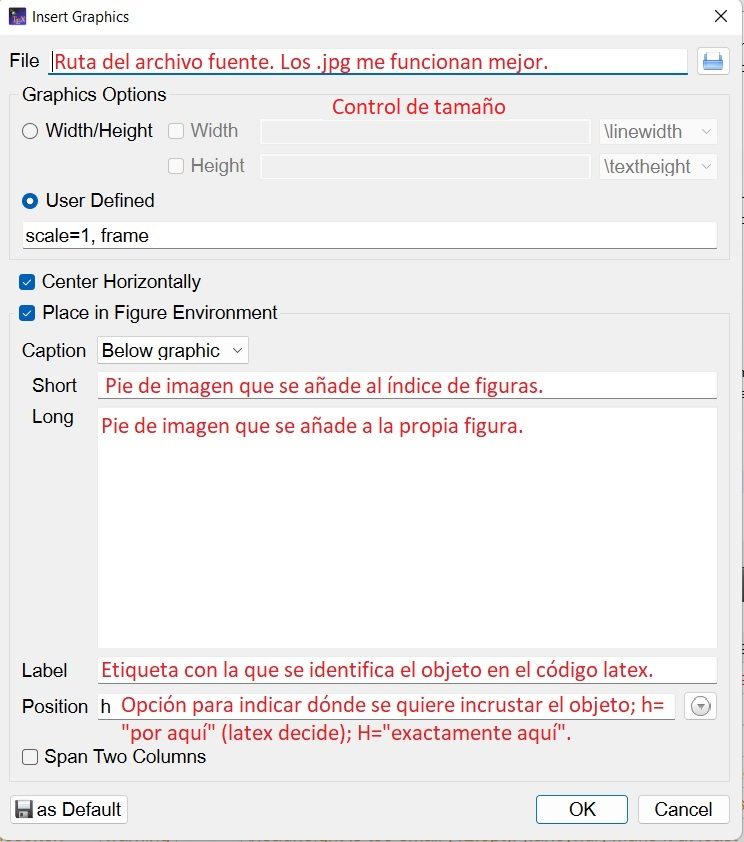
\includegraphics[scale=.65, frame]{cuerpo/cap-objetos/imagenes/auxiliar-imagenes}
	\caption[Interfaz del asistente de imágenes de TeXstudio.]{Interfaz del asistente de imágenes de TeXstudio. En rojo notas sobre algunos campos que permiten personalizar la imagen.}
	\label{fig:auxiliar-imagenes}
\end{figure}
%
\section{Pie de figura}
La configuración del pie de la figura se realiza en el archivo de configuración \textit{02-paquetes.tex}, en las líneas que se muestran en la figura \ref{fig:personalizacion-pies}. Se emplea el paquete \href{https://www.ctan.org/pkg/caption}{\textit{caption}}.

\begin{figure}[h]
	\centering
	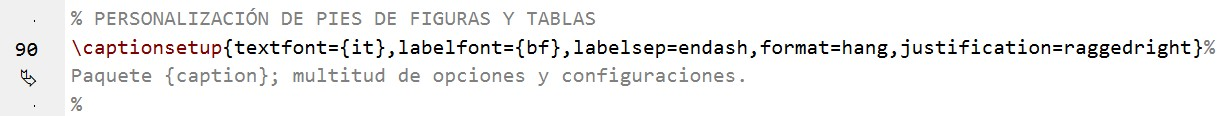
\includegraphics[width=1\textwidth, frame]{cuerpo/cap-objetos/imagenes/personalizacion-pies}
	\caption[Configuración de pies de objetos.]{Configuración de pies de objetos. El comando mostrado se emplea para configurar los pies de los objetos tipo \textit{caption}, que incluye figuras, tablas, código importado. Archivo: .../raiz/configuracion/02-paquetes.tex}.
	\label{fig:personalizacion-pies}
\end{figure}
%
\newpage
Se incluyen a continuación ejemplos de disposiciones frecuentes de imágenes; el código empelado es el mostrado en el fragmento \ref{cod-fig-ejemplo}.
\lstinputlisting[frame={single}, language={[AlLaTeX]TeX}, label={cod-fig-ejemplo}, caption=Código para las imágenes ejemplo \ref{fig:robotdevil} a \ref{fig:grafico-multiple}]{cuerpo/cap-objetos/codigos/imagenes-01.txt}.
%
\begin{figure}[H]
	\centering
	
\includegraphics[scale=1.5, frame]{cuerpo/cap-objetos/imagenes/robotdevil.jpg}
	\caption[Imagen simple 1.]{Imagen simple 1. Una única imagen.}
	\label{fig:robotdevil}
\end{figure}
%
\begin{figure}[H]
	\centering
	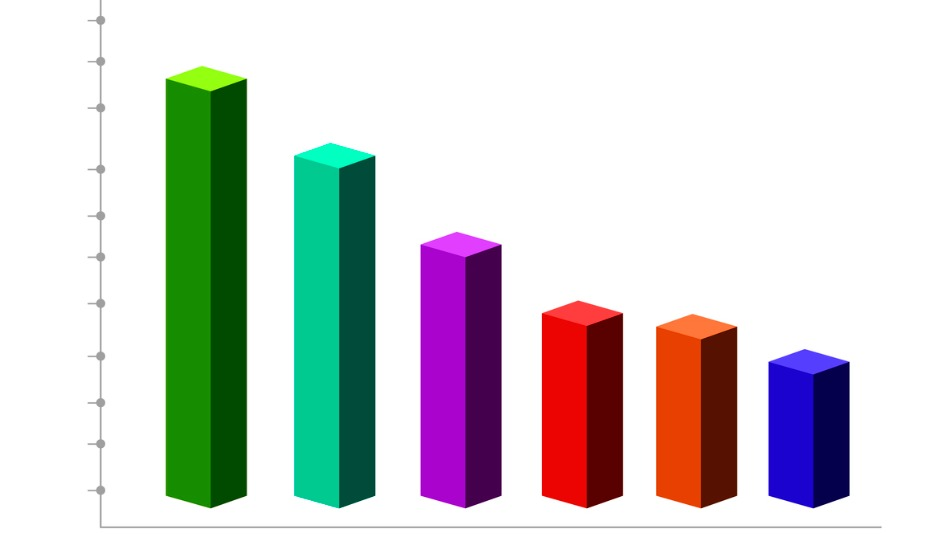
\includegraphics[scale=.5]{cuerpo/cap-objetos/imagenes/grafico-de-barras}
	\caption[Gráfico simple 1.]{Gráfico simple 1. Un gráfico, con fondo blanco y sin borde en la imagen fuente.}
	\label{fig:grafico-de-barras}
\end{figure}
%
\begin{figure}[H]
	\centering
	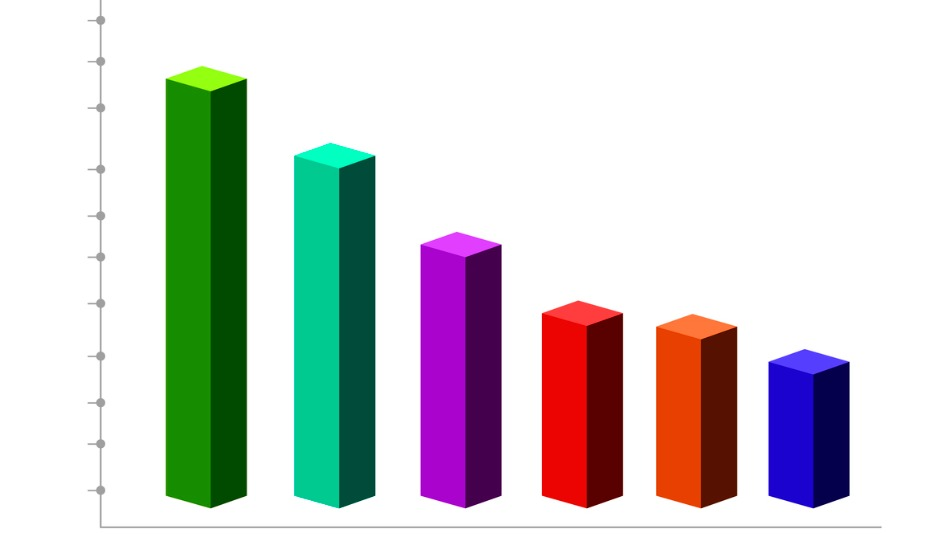
\includegraphics[scale=.5, frame]{cuerpo/cap-objetos/imagenes/grafico-de-barras}
	\caption[Gráfico simple 2.]{Gráfico simple 2. Un gráfico, con fondo blanco y sin borde en la imagen fuente, pero con el borde añadido en \LaTeX; por defecto esta plantilla añade el borde.}
	\label{fig:grafico-de-barras-bis}
\end{figure}
%
\begin{figure}[H]
	\centering
	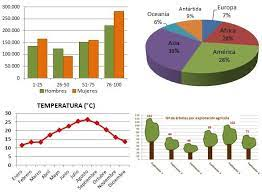
\includegraphics[scale=1, frame]{cuerpo/cap-objetos/imagenes/grafico-multiple}
	\caption[Gráfico simple 3.]{Gráfico simple 3. Un gráfico cuya imagen fuente es un collage de varias imágenes, por lo que en realidad es un único objeto.}
	\label{fig:grafico-multiple}
\end{figure}
%
\section{Subfiguras}
Se pueden crear figuras compuestas de subfiguras.
\begin{figure}[H]
	\centering
	\begin{subfigure}[b]{0.45\textwidth}
		\centering
		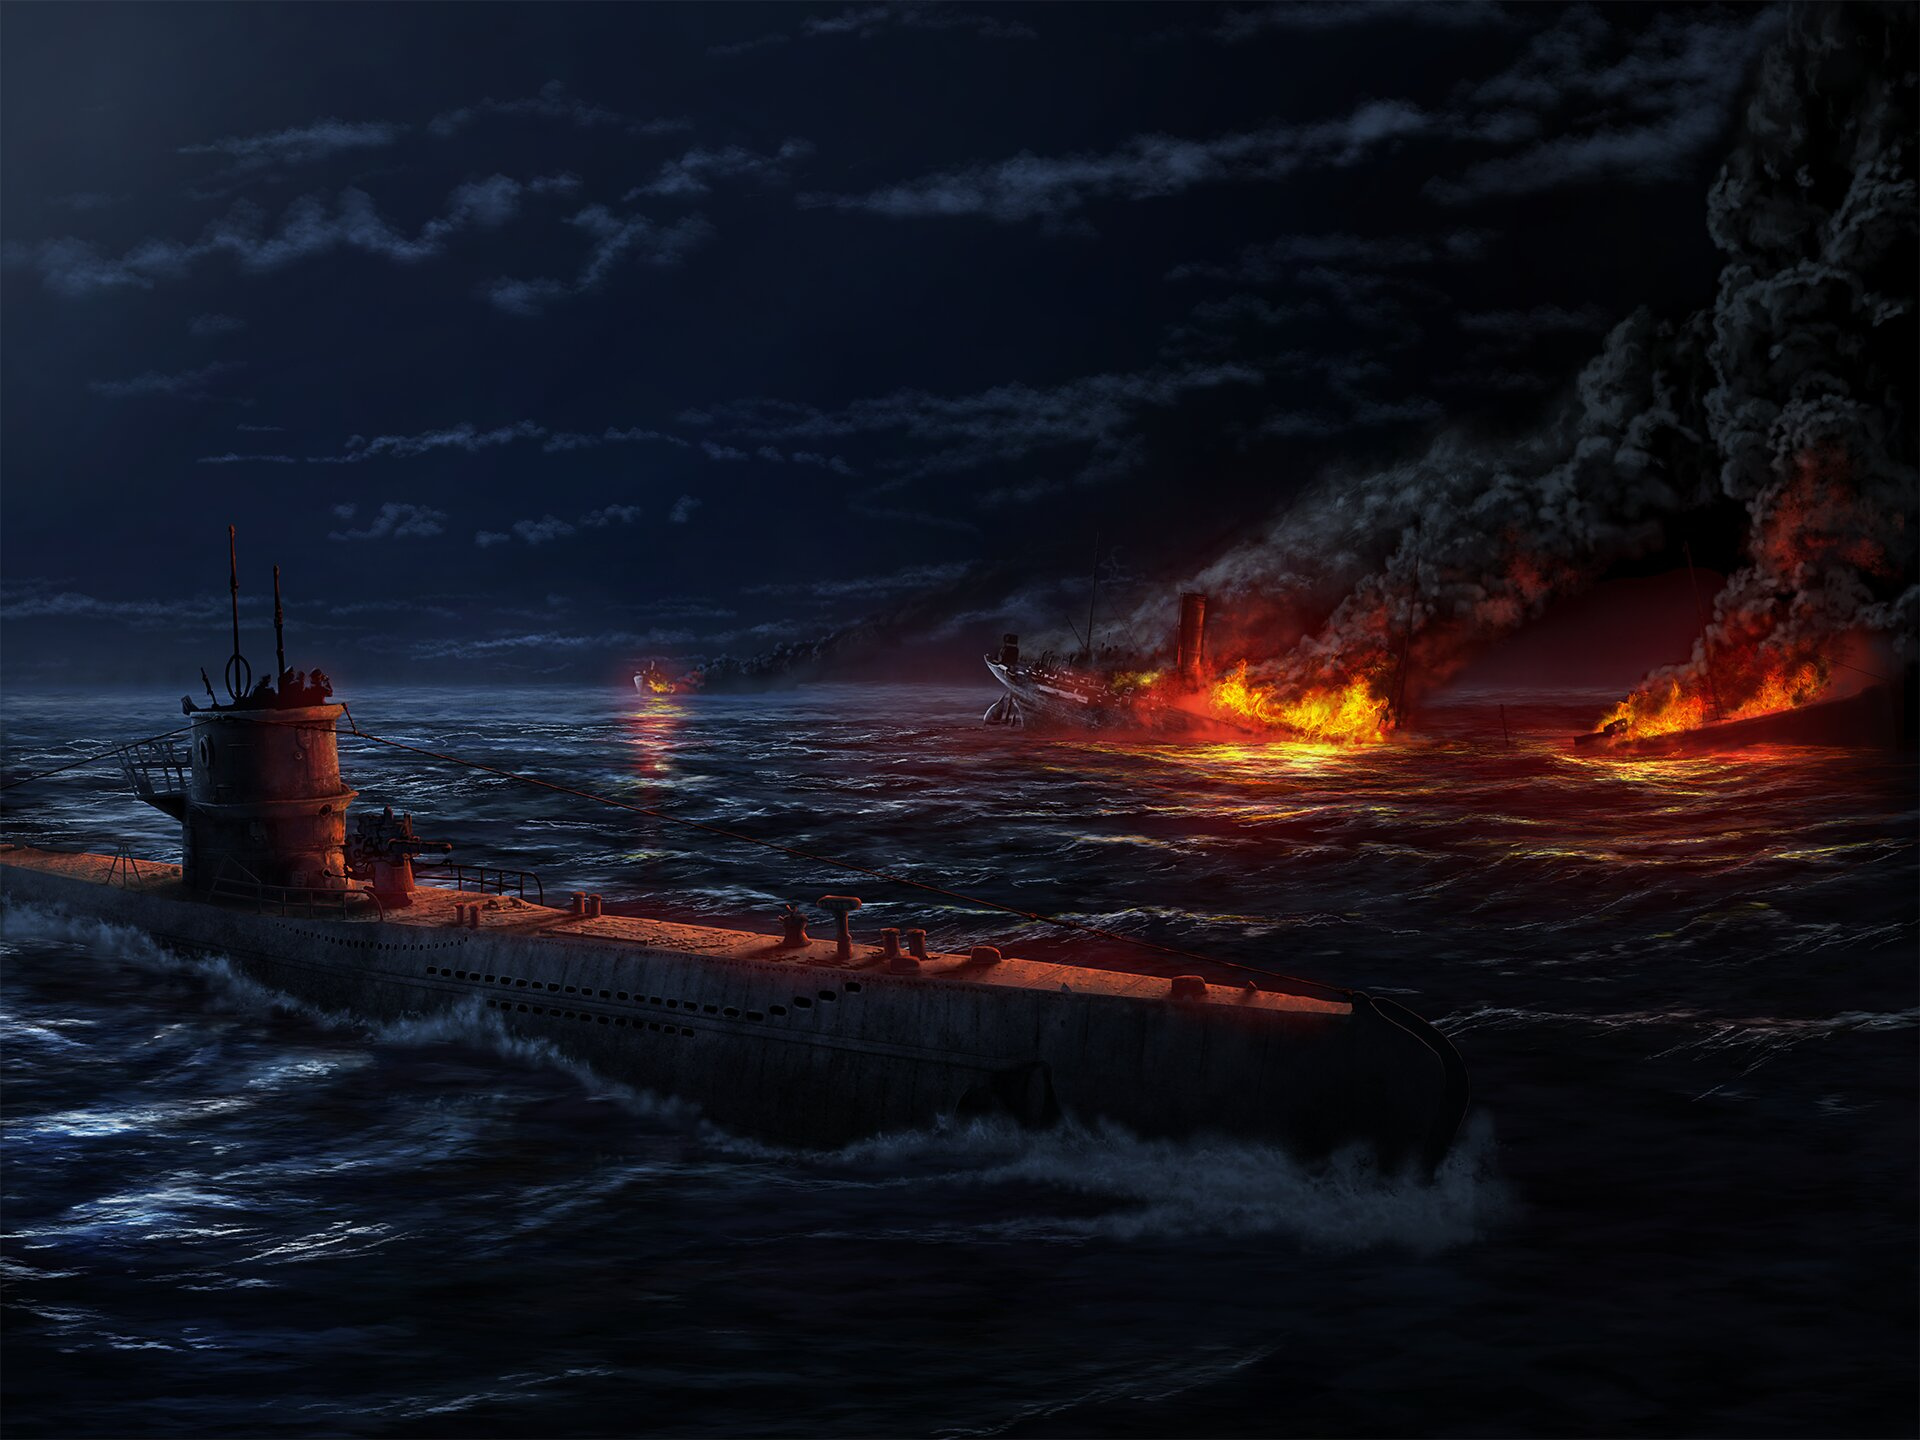
\includegraphics[width=\textwidth]{cuerpo/cap-objetos/imagenes/hoi4-convoy-raiding}
		\caption{Uboat atacando convoy.}
		\label{fig:hoi4-convoy-raiding}
	\end{subfigure}
	%
	\begin{subfigure}[b]{0.45\textwidth}
		\centering
		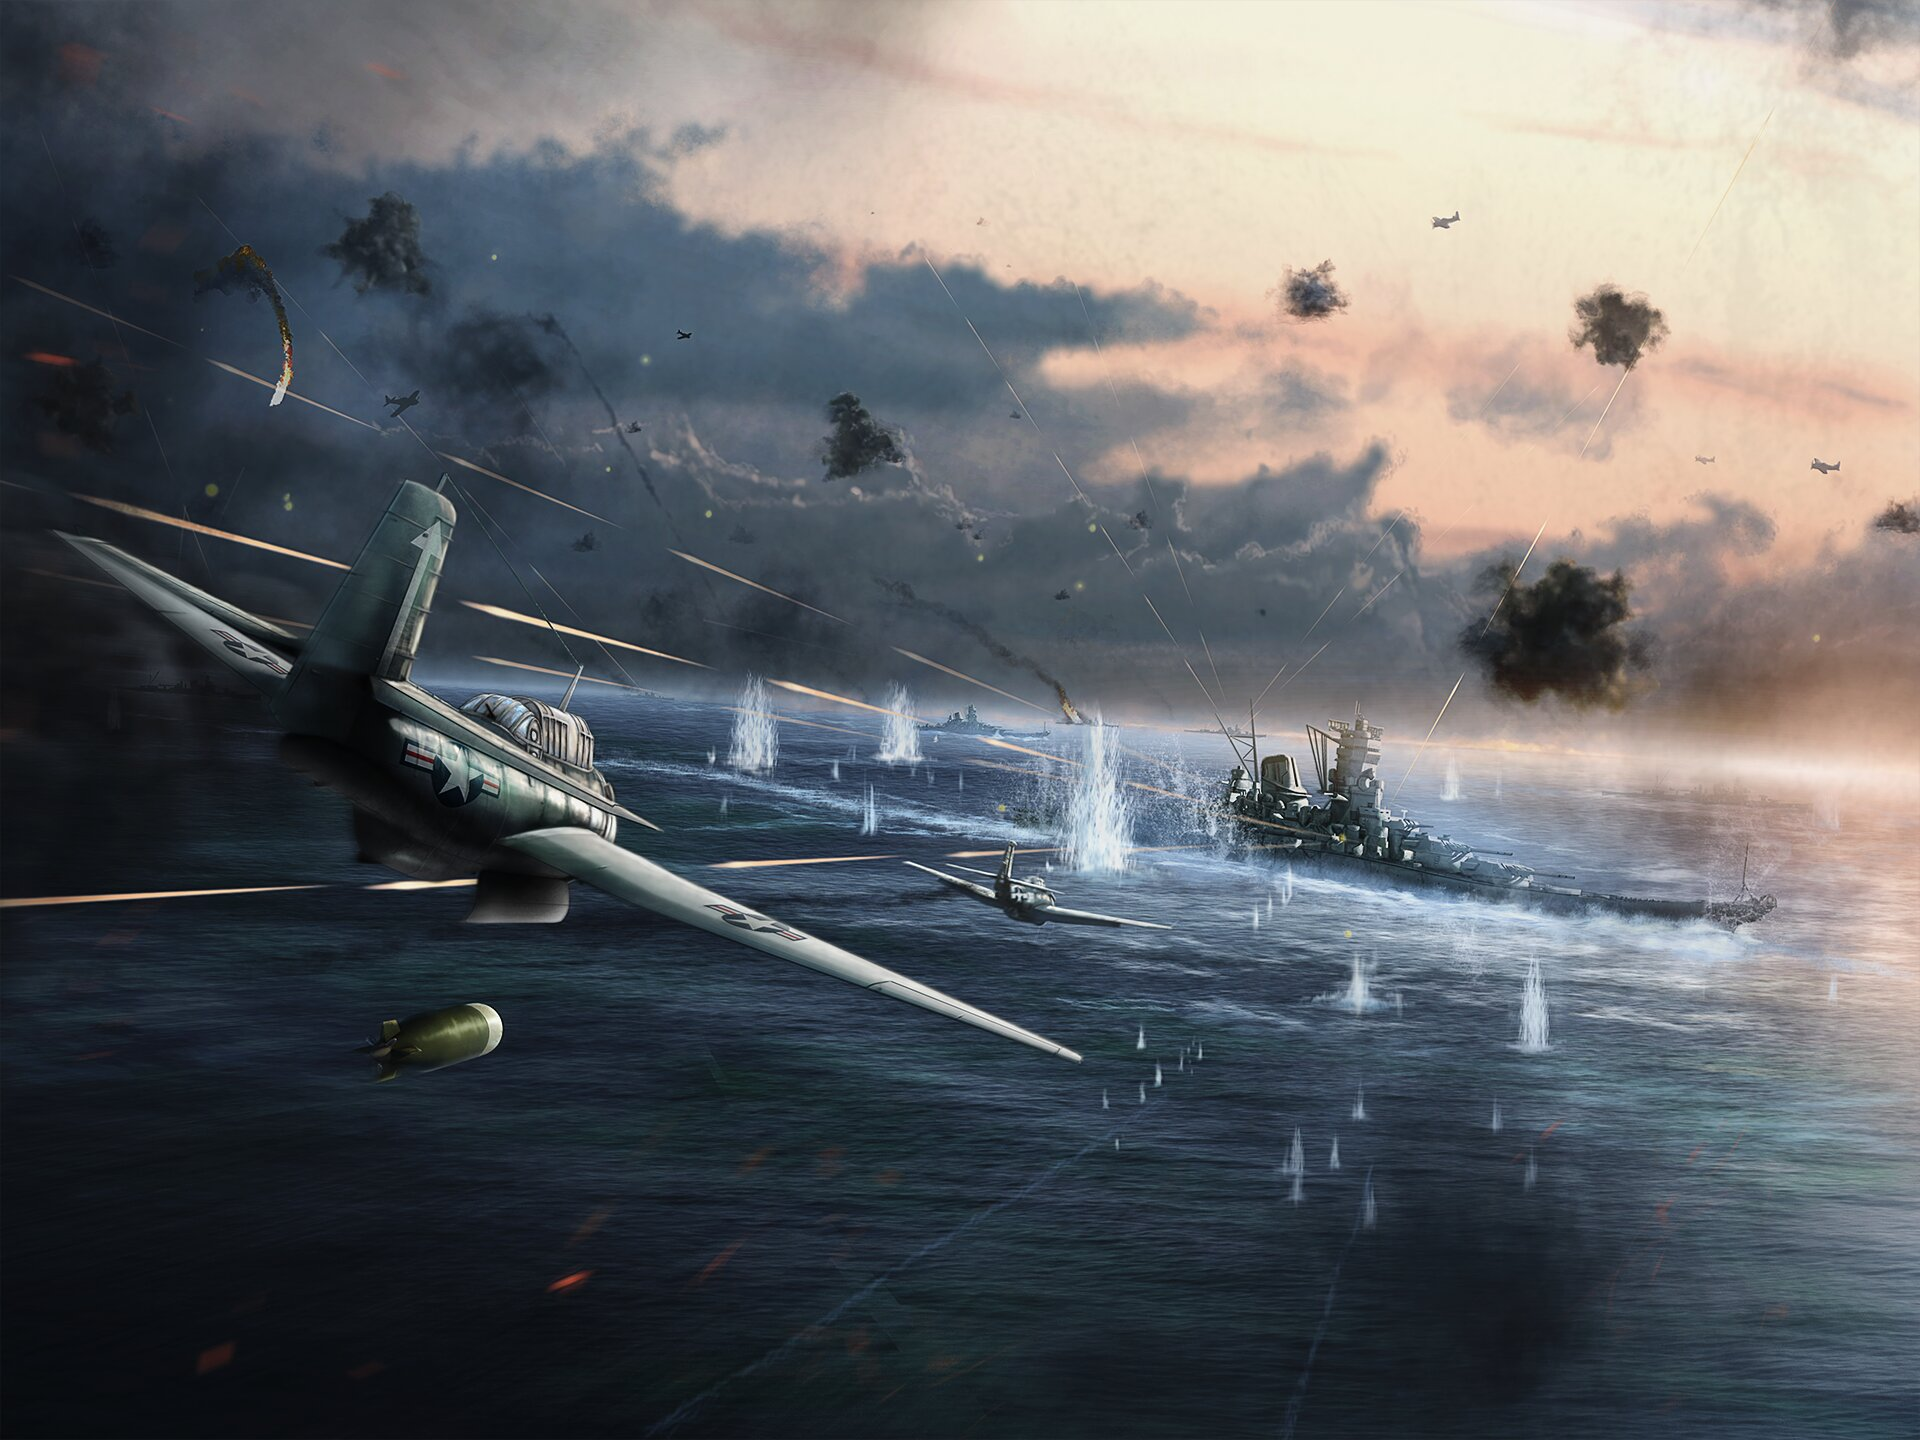
\includegraphics[width=\textwidth]{cuerpo/cap-objetos/imagenes/hoi4-aeronaval-battle}
		\caption{Torpedero naval atacando acorazado.}
		\label{fig:hoi4-aeronaval-battle}
	\end{subfigure}
	\caption[Figura con 2 subfiguras - ejemplo 1.]{Figura con 2 subfiguras - ejemplo 1. Figuras alineadas inferiormente y en una misma linea. Batallas aeronavales de la Segunda Guerra Mundial. Fuente: \cite{hoi4}.}
	\label{fig:aeronavales}
\end{figure}
%
%\newpage
\lstinputlisting[frame={single}, language={[AlLaTeX]TeX}, label={cod-fig:aeronavales}, caption=Código de la figura \ref{fig:aeronavales}.]{cuerpo/cap-objetos/codigos/subfigura1.txt}
%
\begin{figure}[H]
	\centering
	\begin{subfigure}[b]{1\textwidth}
		\centering
		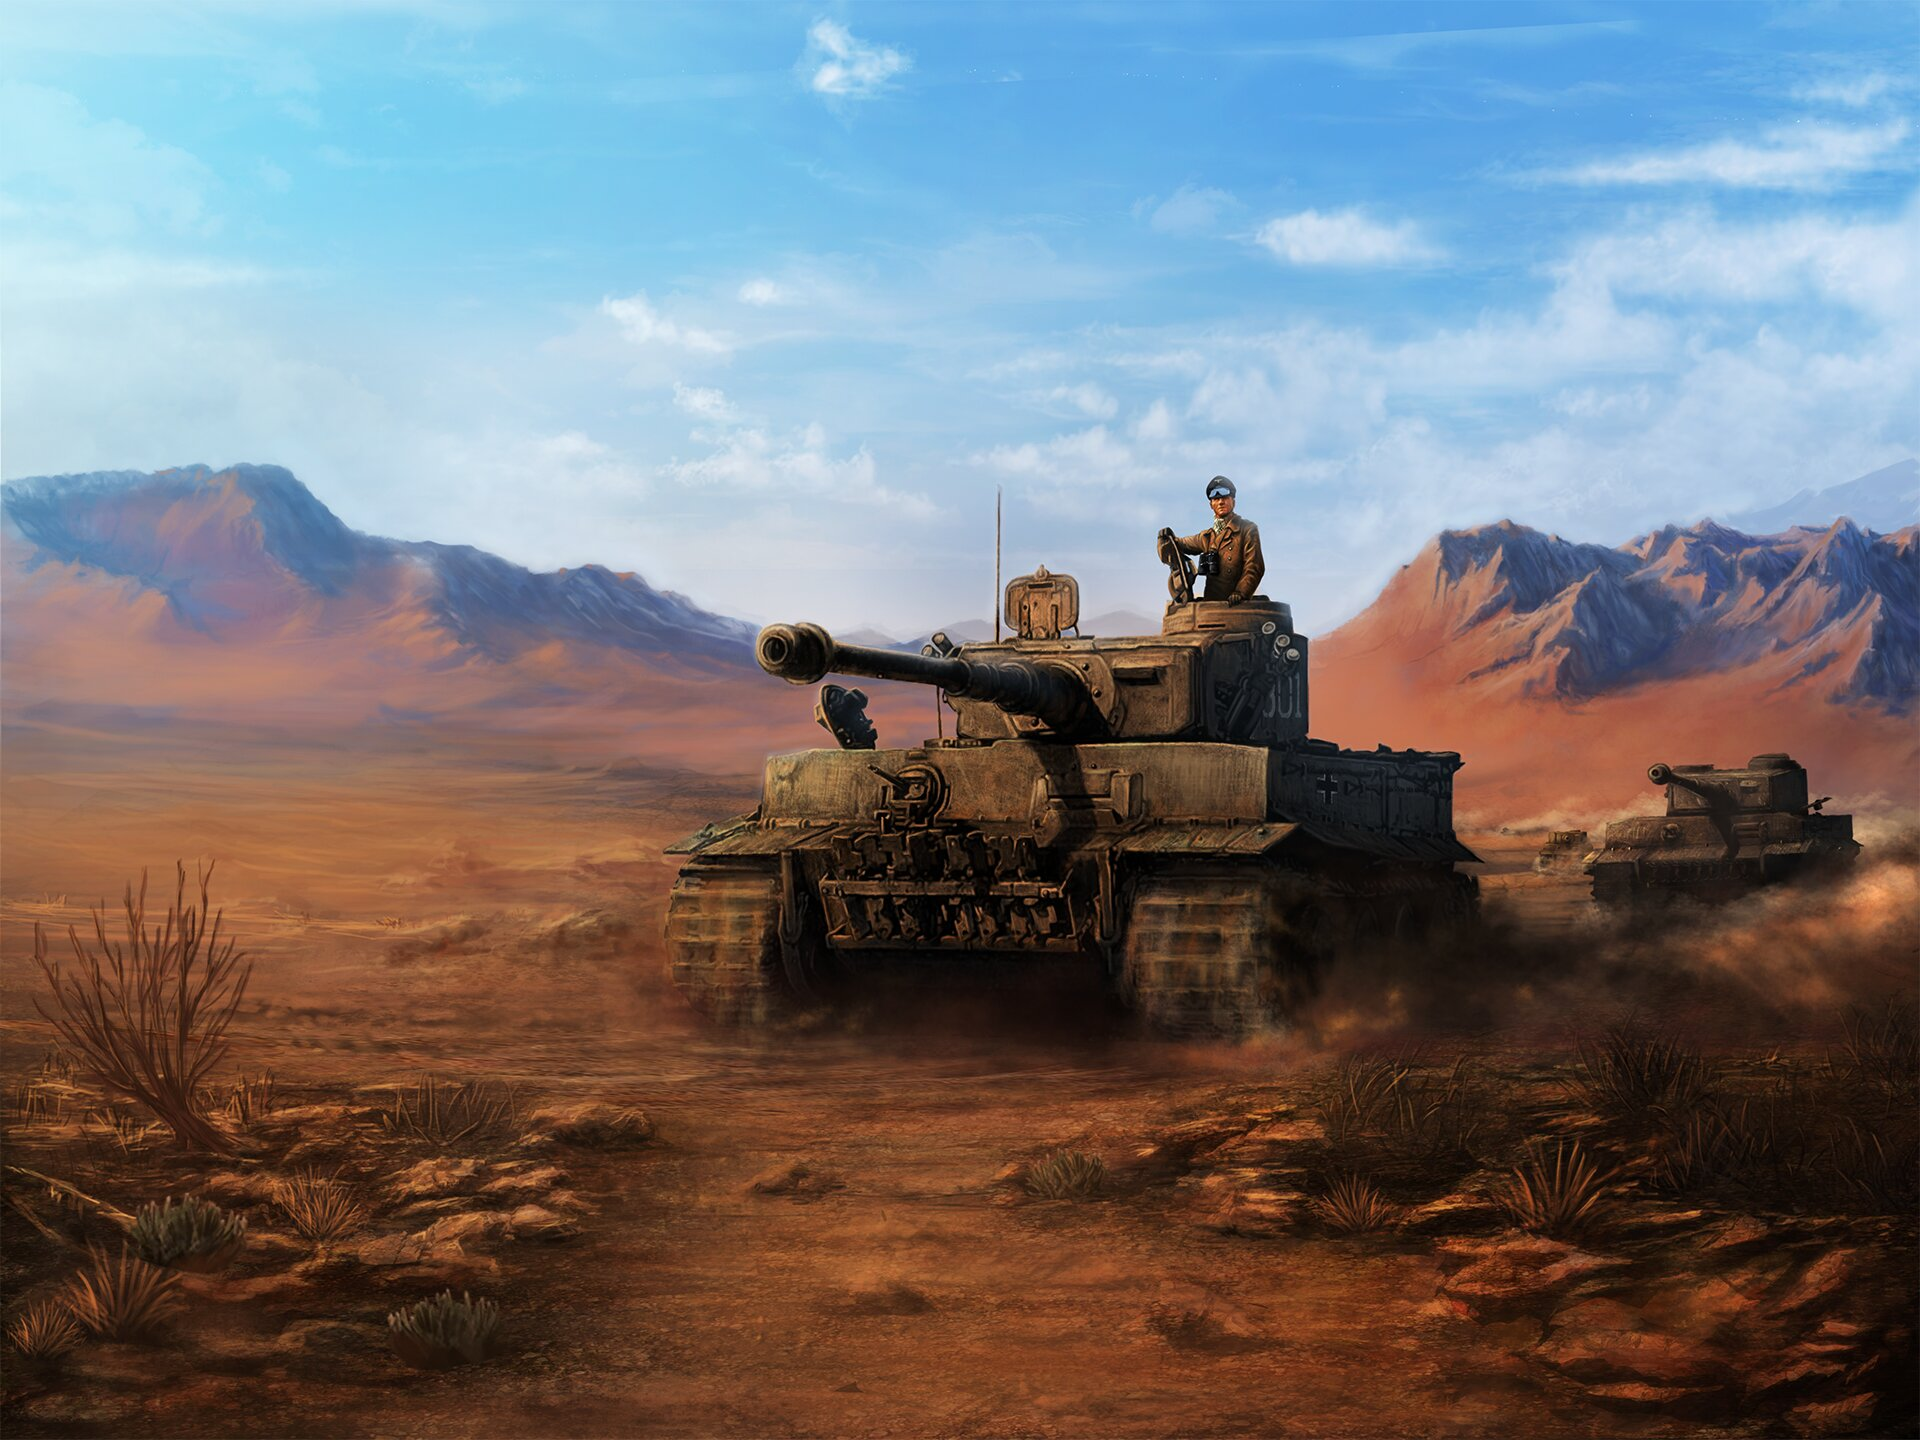
\includegraphics[width=0.75\textwidth]{cuerpo/cap-objetos/imagenes/hoi4-afrika-korps}
		\caption{Afrika korps.}
		\label{fig:hoi4-afrika-korps}
	\end{subfigure}
	%
	\begin{subfigure}[b]{1\textwidth}
		\centering
		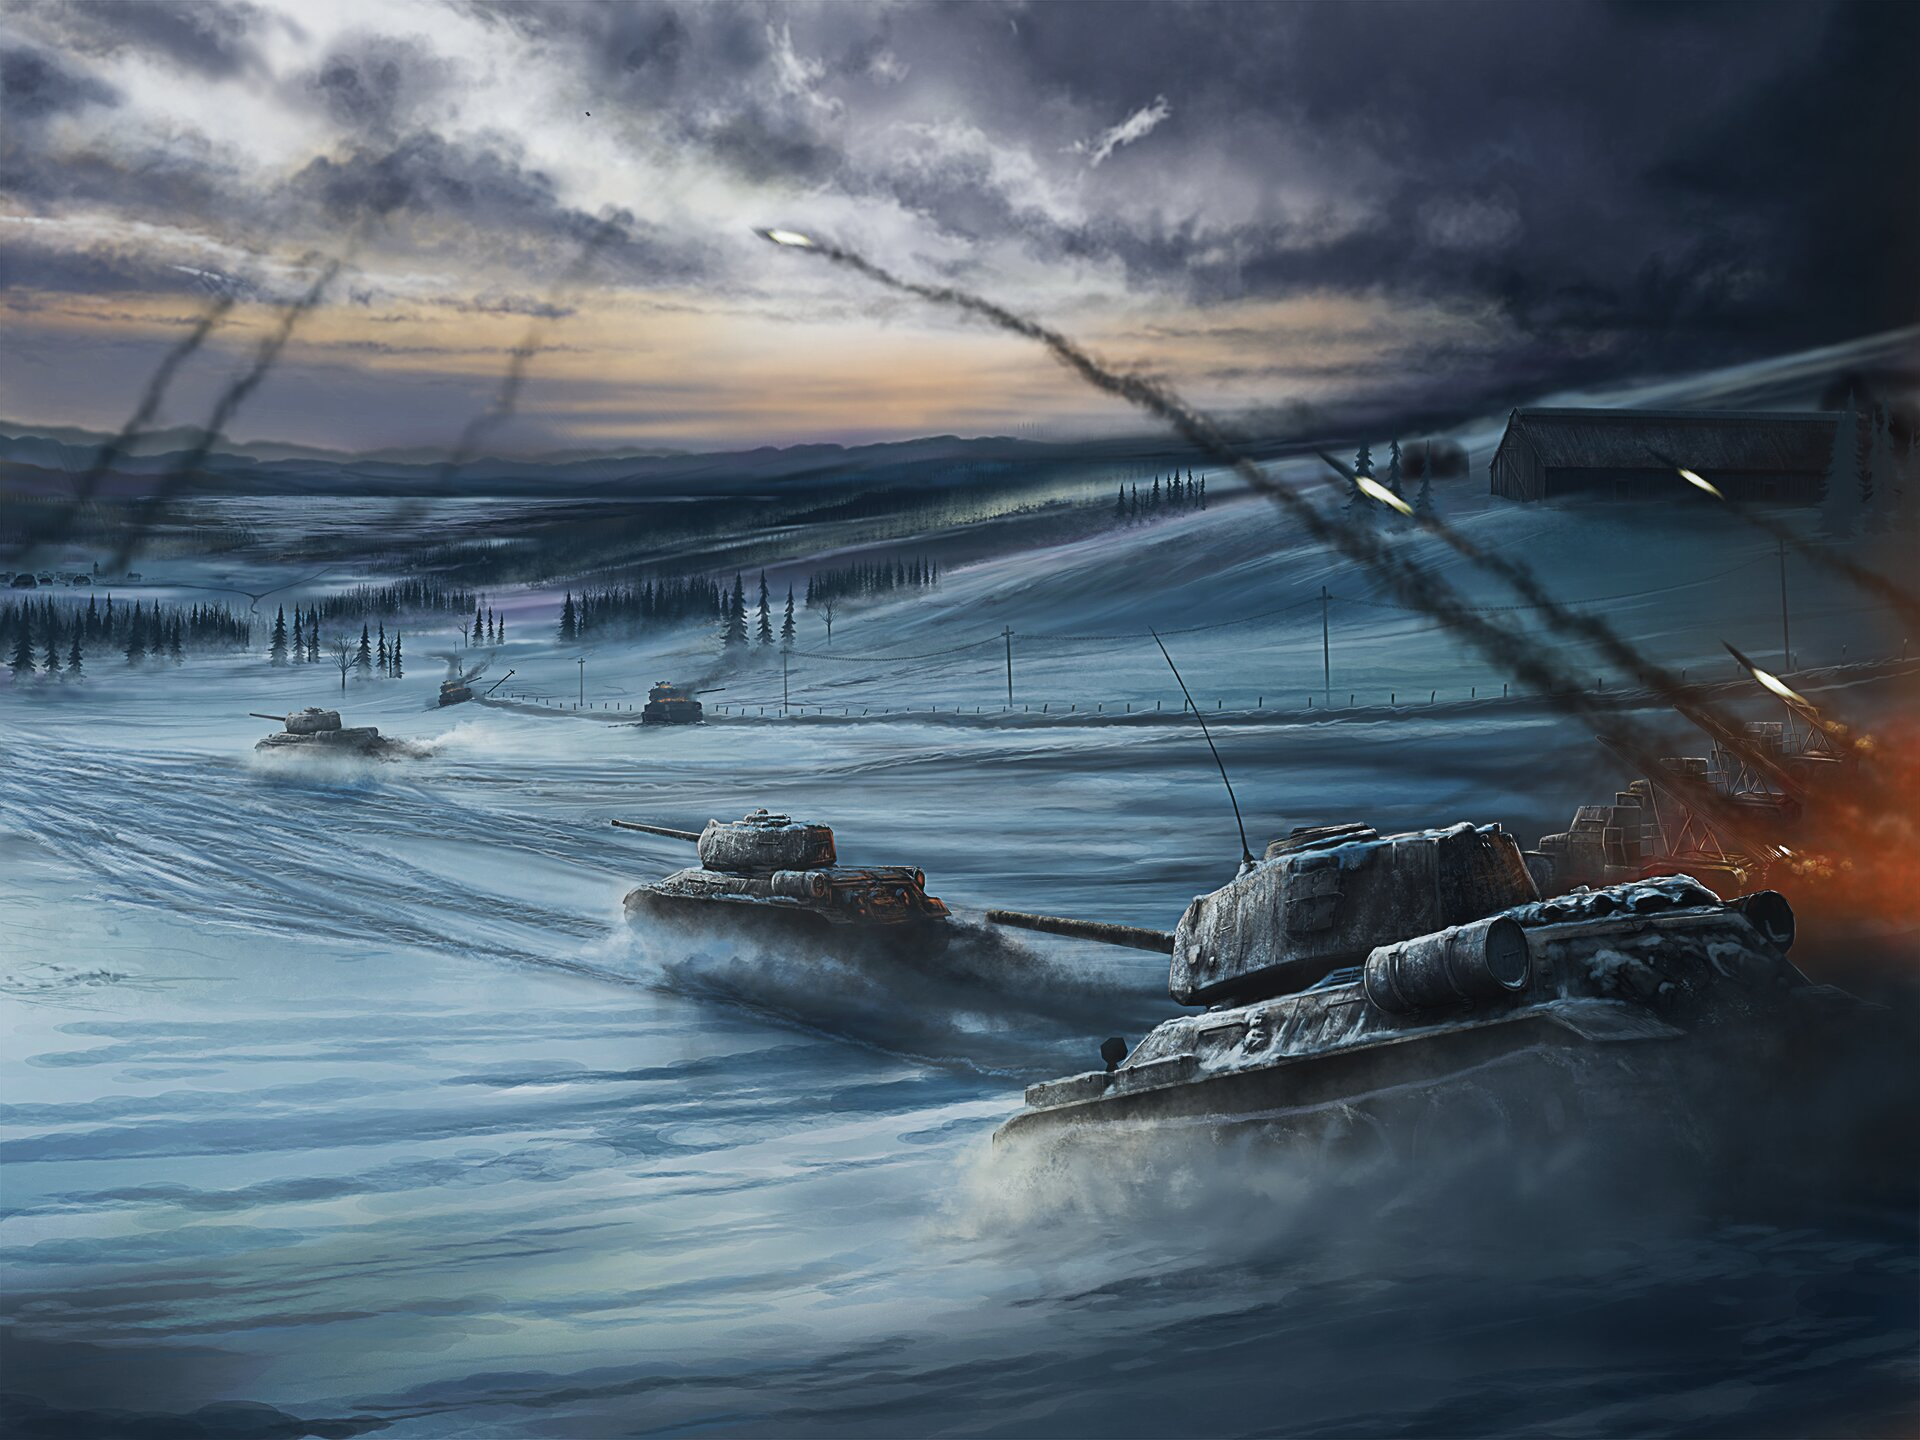
\includegraphics[width=0.75\textwidth]{cuerpo/cap-objetos/imagenes/hoi4-soviet-tanks}
		\caption{Tanques soviéticos.}
		\label{fig:hoi4-soviet-tanks}
	\end{subfigure}
	%
	\caption[Figura con 2 subfiguras - ejemplo 2.]{Figura con 2 subfiguras - ejemplo 2. Figuras alineadas inferiormente y en diferentes lineas. Tanques en la Segunda Guerra Mundial. Fuente: \cite{hoi4}.}
	\label{fig:tanques}
\end{figure}
%
\newpage
\lstinputlisting[frame={single}, language={[AlLaTeX]TeX}, label={cod-fig:tanques}, caption=Código de la figura \ref{fig:tanques}.]{cuerpo/cap-objetos/codigos/subfigura2.txt}
%
\begin{figure}[H]
	\centering
	\begin{subfigure}[b]{0.45\textwidth}
		\centering
		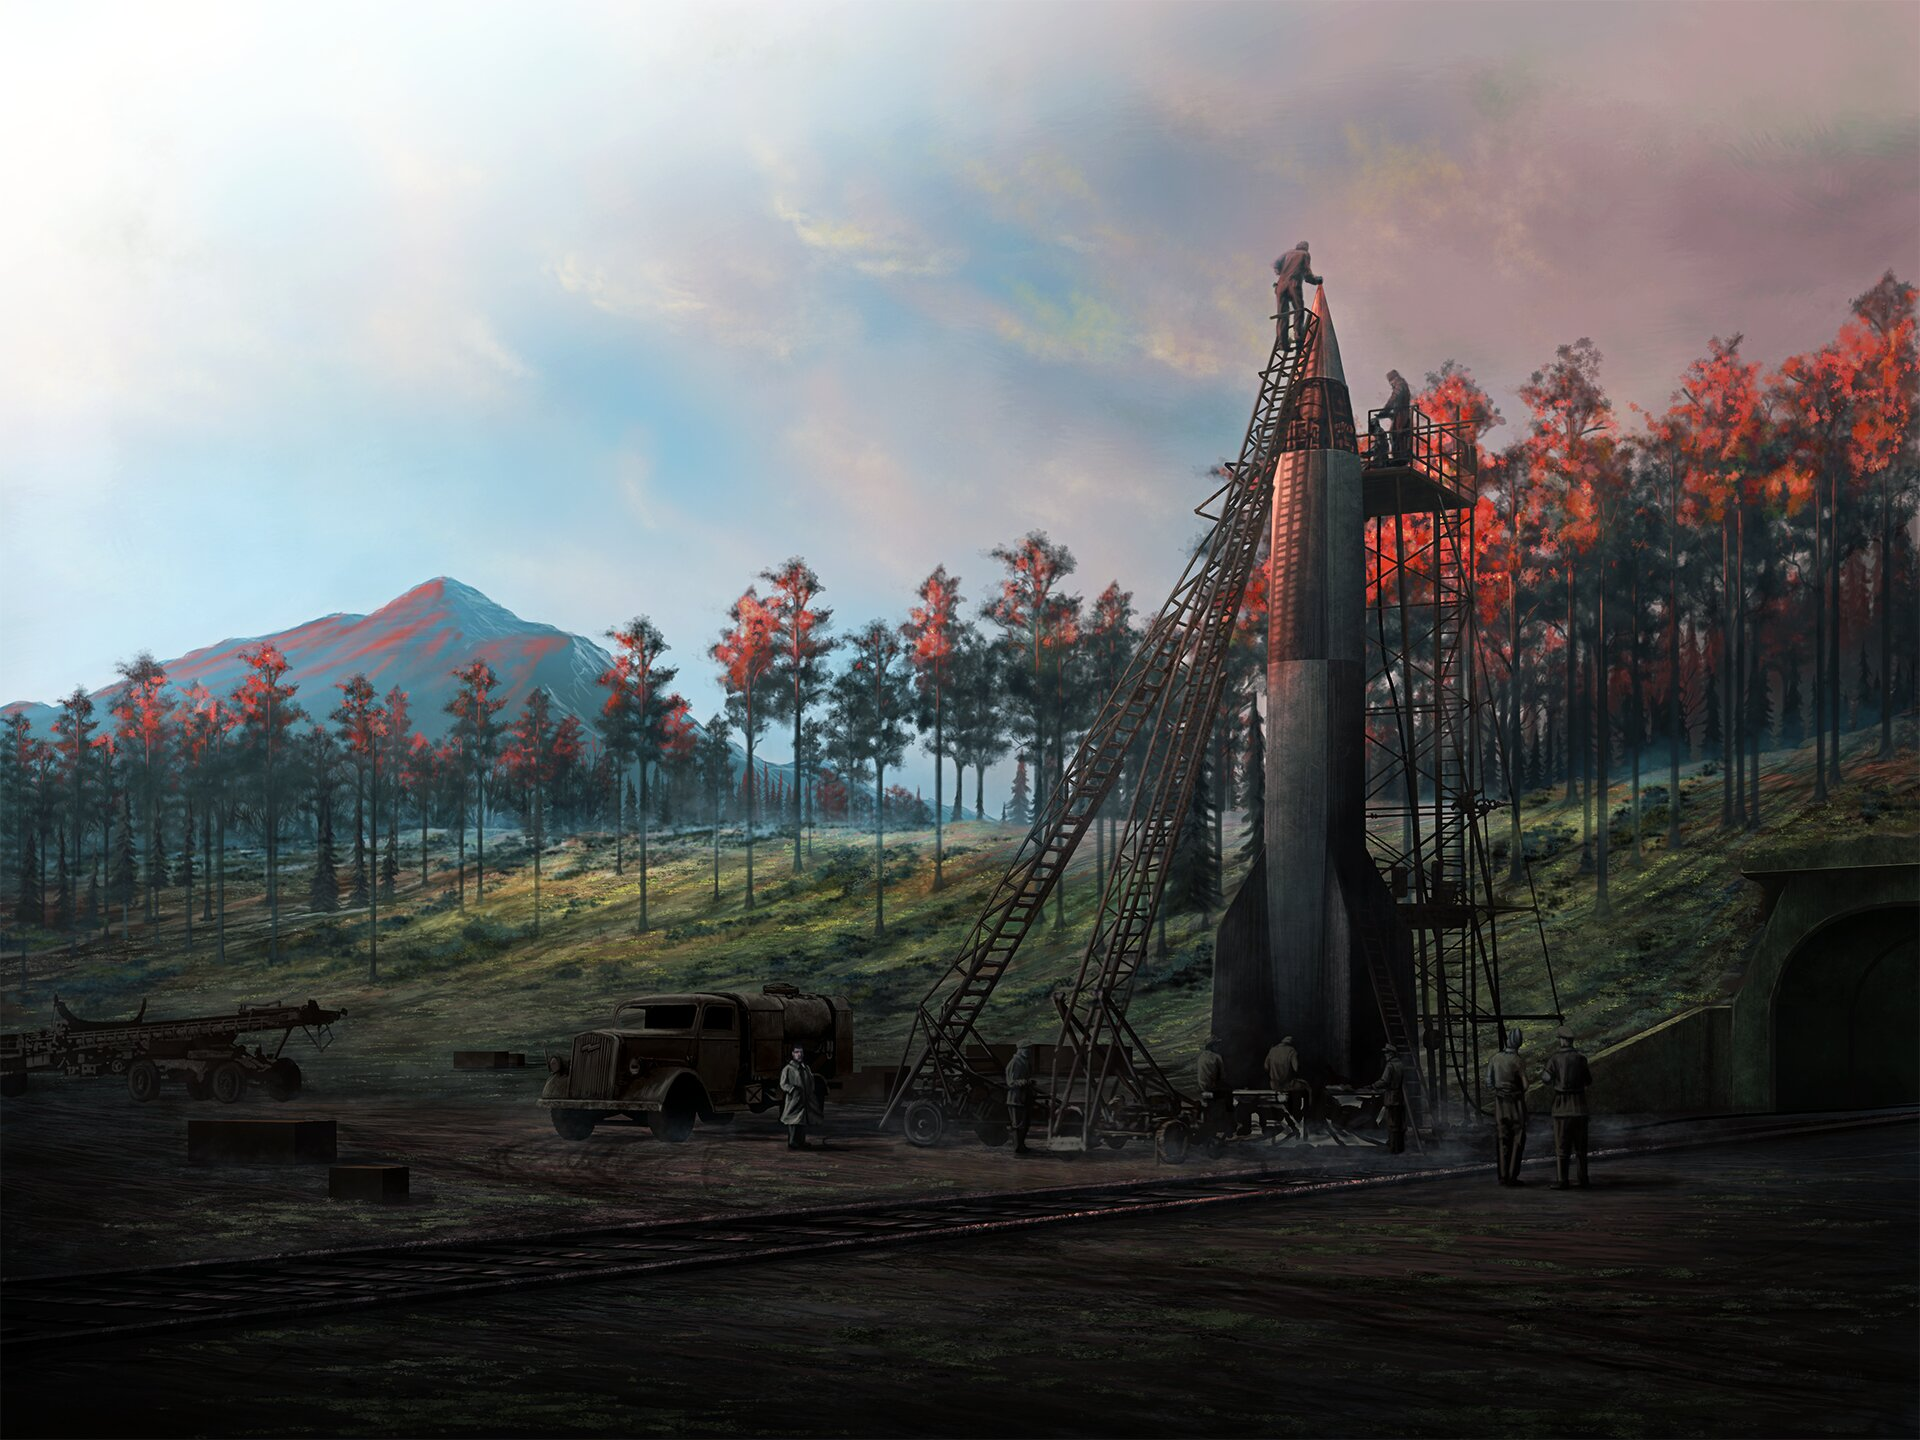
\includegraphics[width=\textwidth, frame]{cuerpo/cap-objetos/imagenes/hoi4-v2}
		\caption{V2.}
		\label{fig:hoi4-v2}
	\end{subfigure}
	%
	\begin{subfigure}[b]{0.45\textwidth}
		\centering
		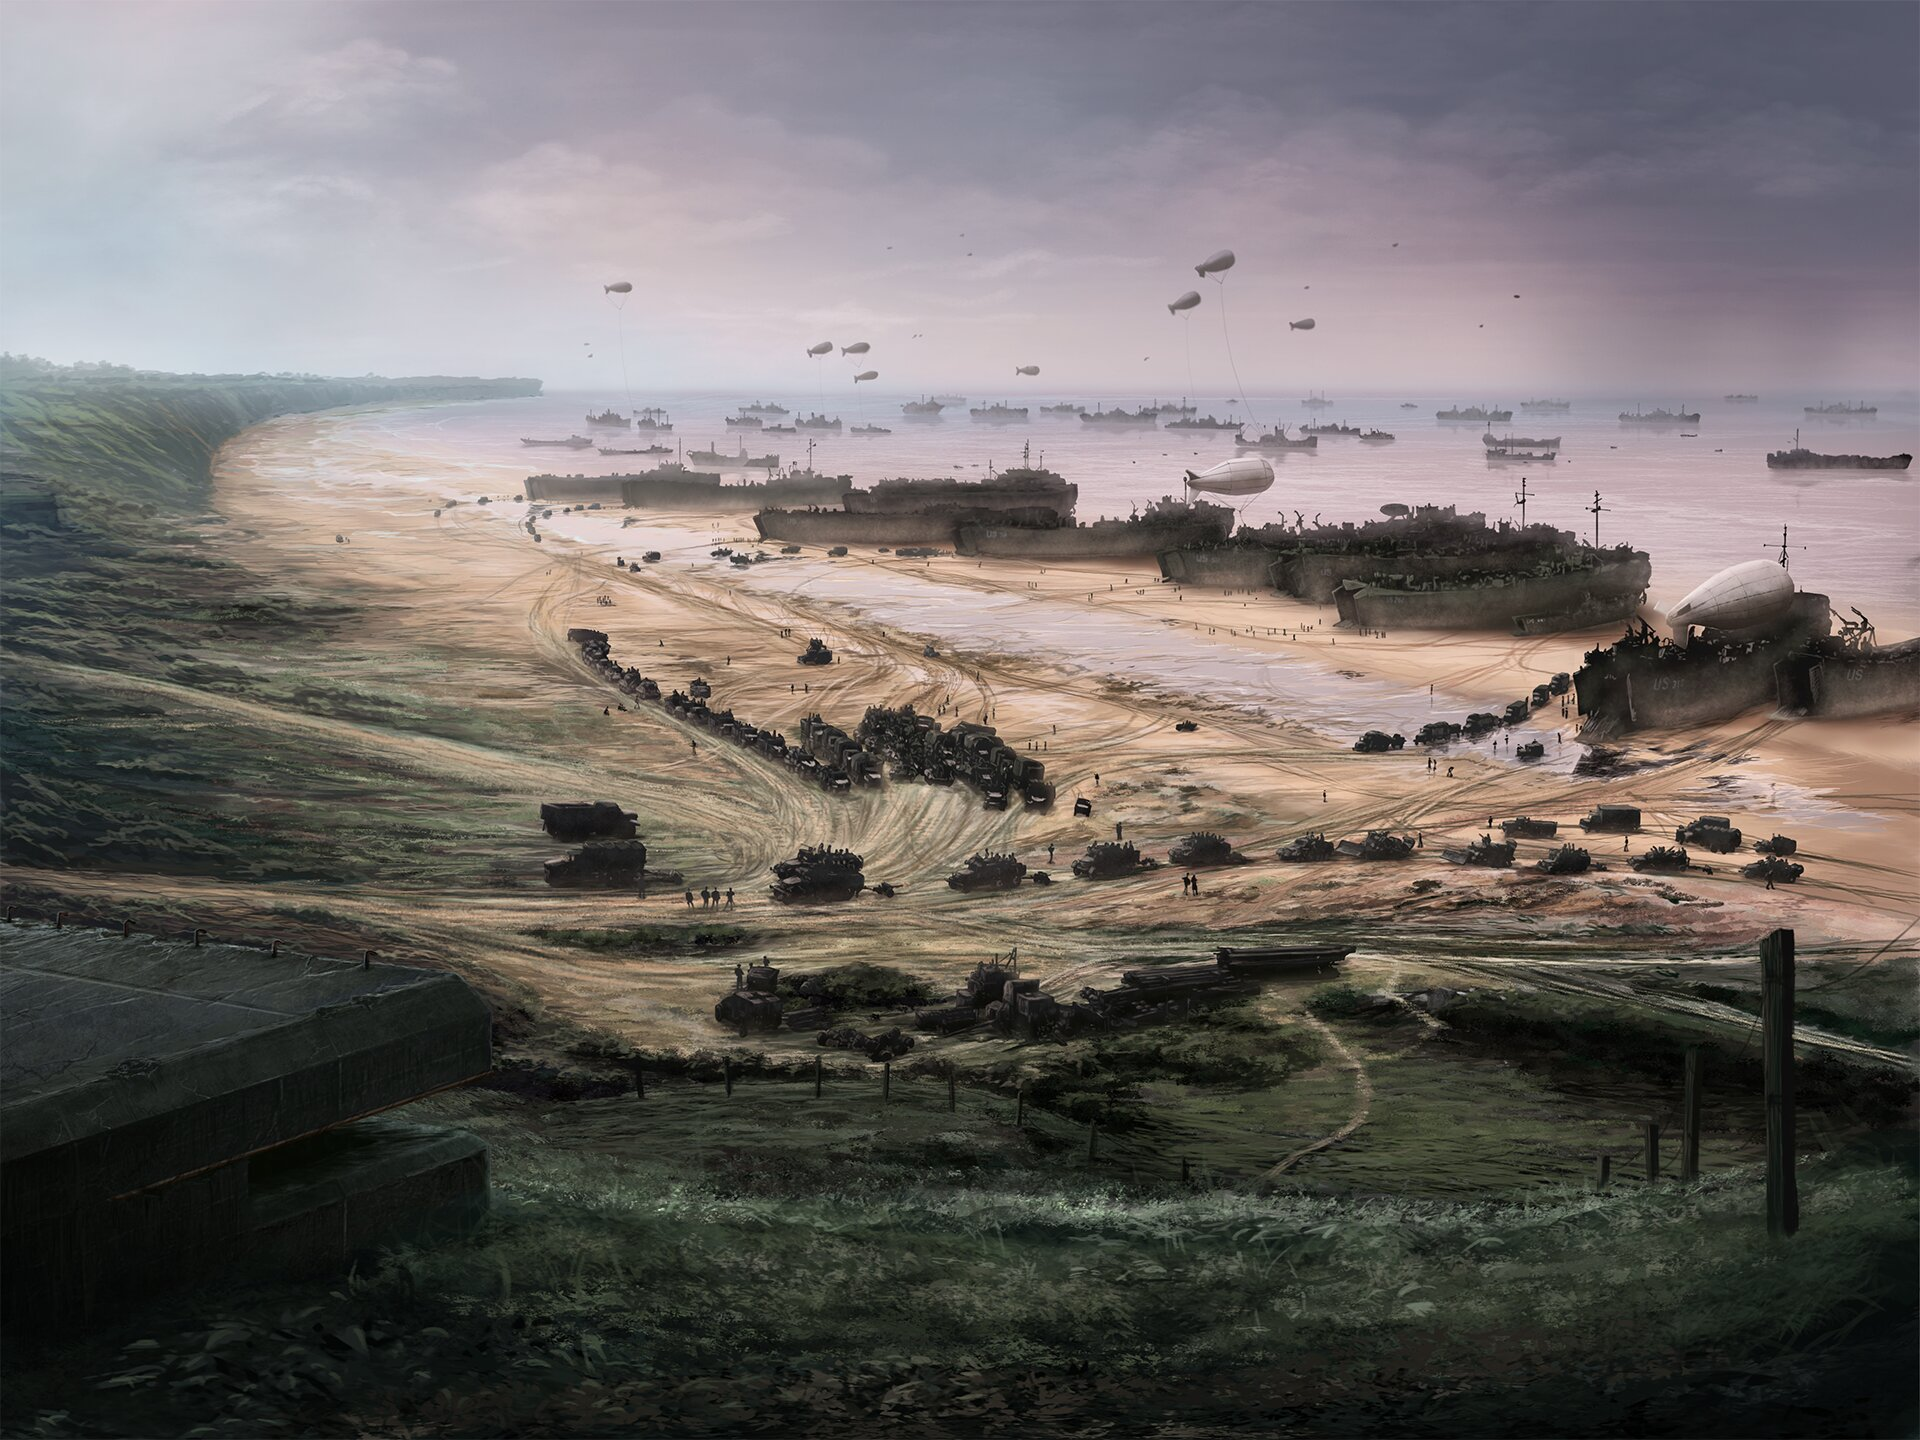
\includegraphics[width=\textwidth, frame]{cuerpo/cap-objetos/imagenes/hoi4-normandy-landing}
		\caption{Desembarco en Normandía.}
		\label{fig:hoi4-normandia}
	\end{subfigure}
	\hfill
		\begin{subfigure}[b]{0.45\textwidth}
		\centering
		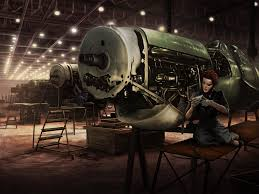
\includegraphics[width=\textwidth, frame]{cuerpo/cap-objetos/imagenes/hoi4-female-worker}
		\caption{Mujer en fábrica de armamento.}
		\label{fig:hoi4-female-worker}
	\end{subfigure}
	%
	\begin{subfigure}[b]{0.45\textwidth}
		\centering
		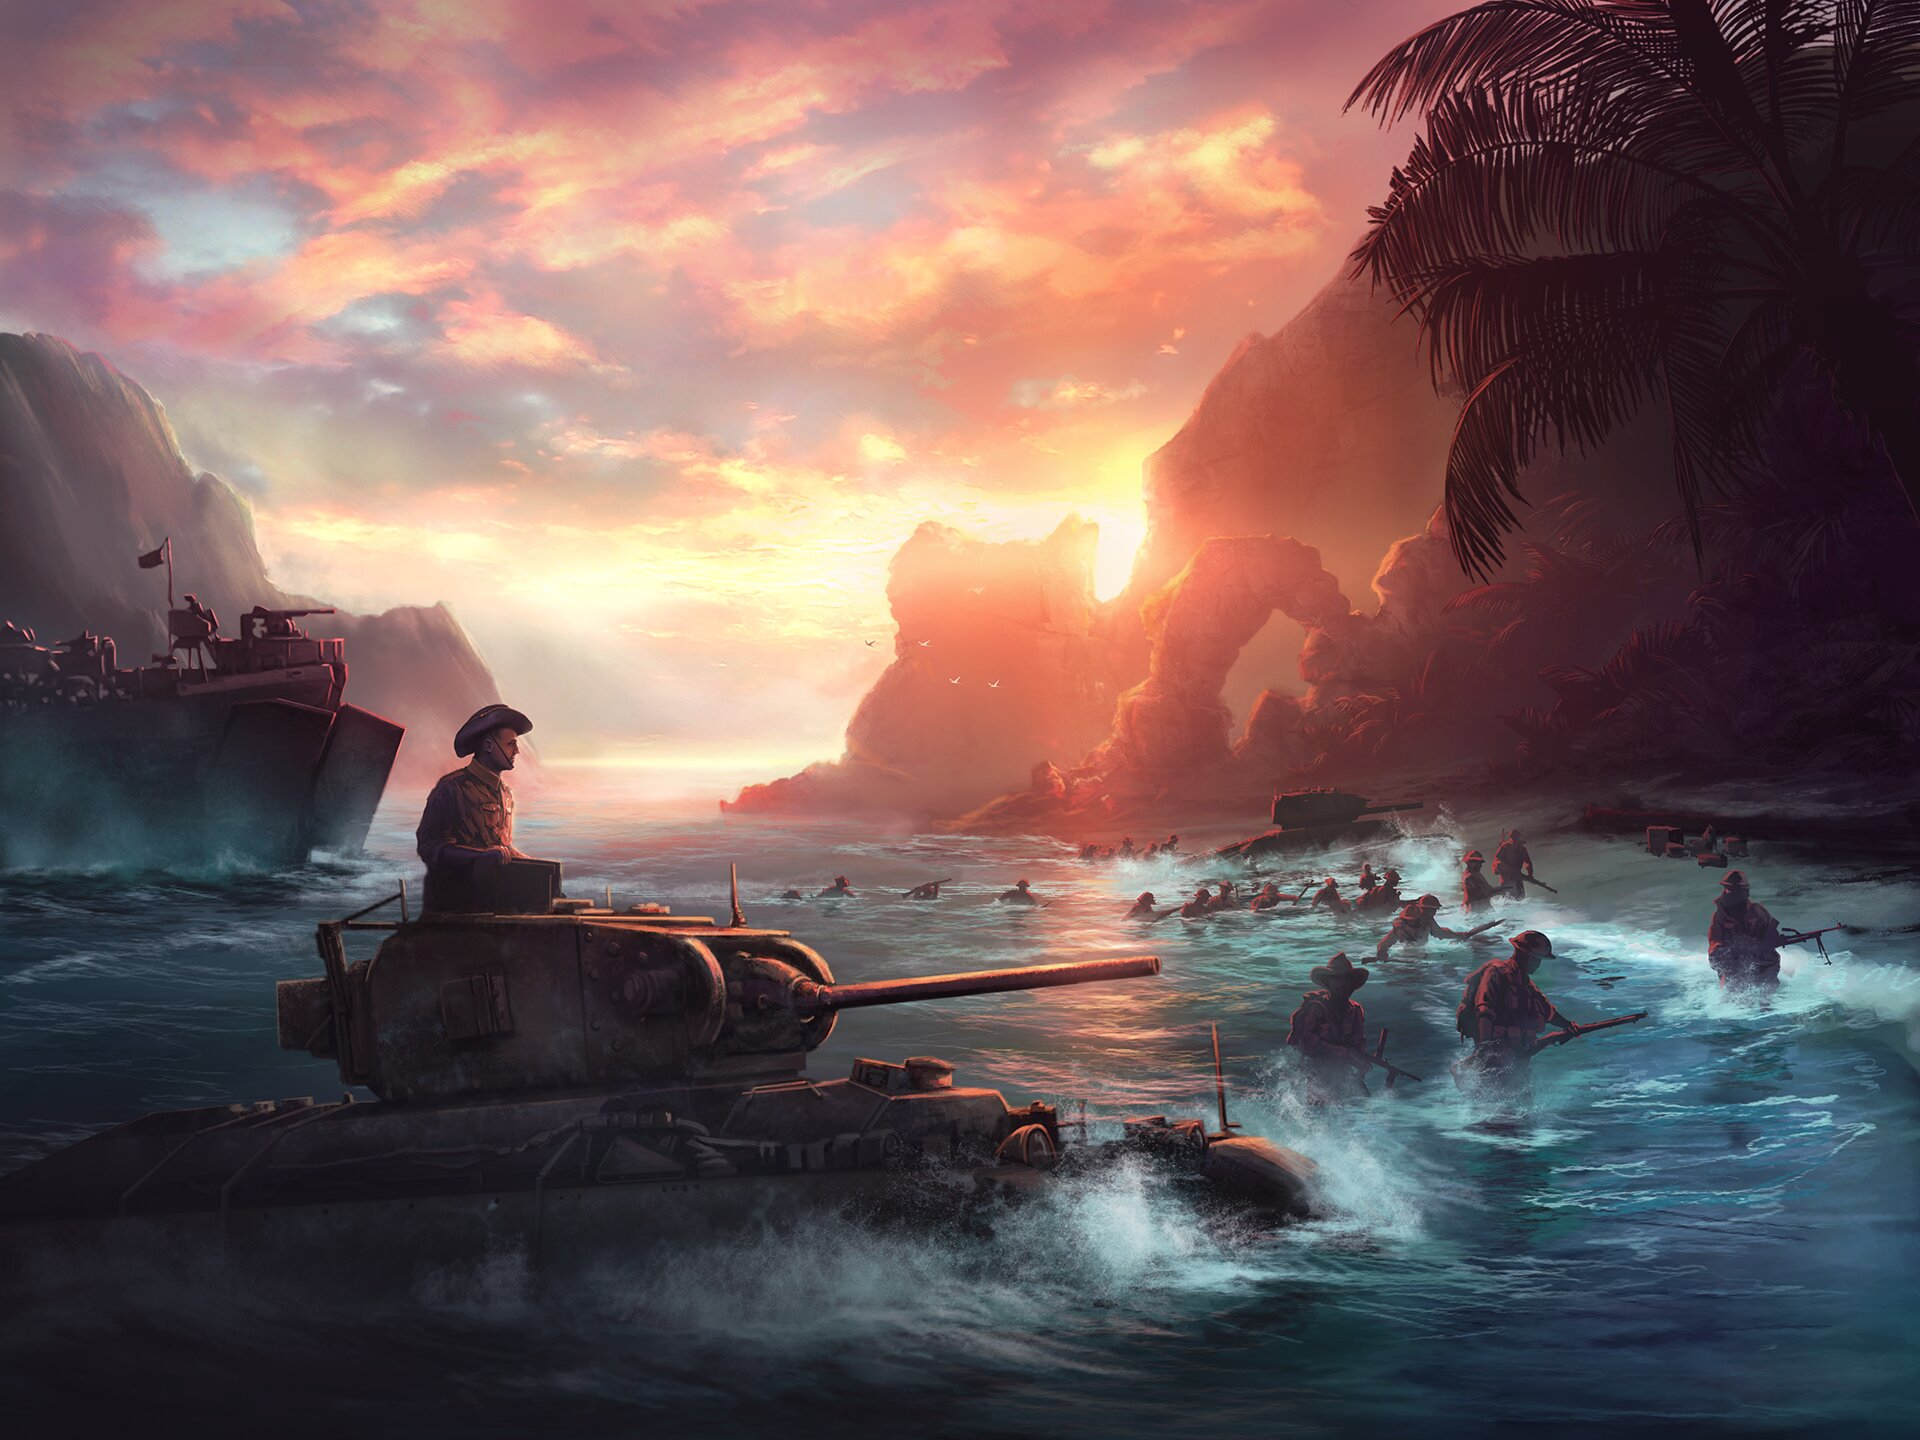
\includegraphics[width=\textwidth, frame]{cuerpo/cap-objetos/imagenes/hoi4-pacific-landing}
		\caption{Desembarco en el Pacífico.}
		\label{fig:hoi4-desembarco-pacifico}
	\end{subfigure}
	%
	\caption[Figura con 4 subfiguras.]{Figura con 4 subfiguras - ejemplo 1. Figuras alineadas inferiormente y en una matriz 2x2. Escenas de la Segunda Guerra Mundial. Fuente: \cite{hoi4}.}
	\label{fig:escenas-ww2}
\end{figure}
%
\newpage
\lstinputlisting[frame={single}, language={[AlLaTeX]TeX}, label={cod-fig:escenas-ww2}, caption=Código de la figura \ref{fig:escenas-ww2}.]{cuerpo/cap-objetos/codigos/subfigura3.txt}
%
\section{Figuras apaisadas}
\begin{figure}[H]
	\centering
	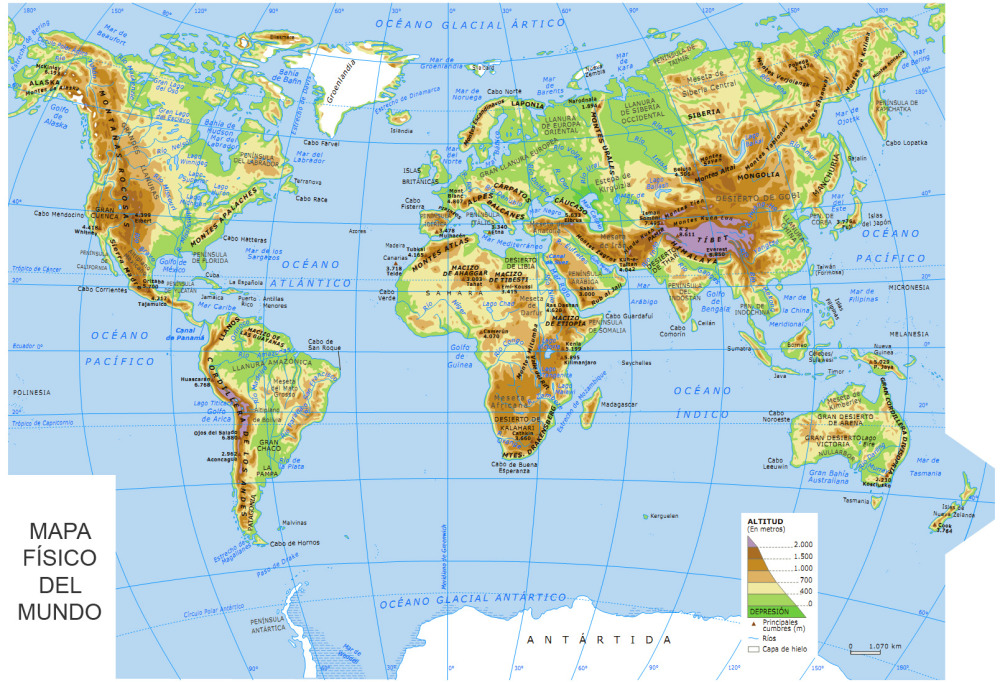
\includegraphics[width=\textwidth, frame]{cuerpo/cap-objetos/imagenes/mapa-fisico}
	\caption[Figura rotada 0.]{Figura rotada 0. Original: esta es la imagen en su posición original, con el tamaño ajustado al ancho de linea.}
	\label{fig:mapa-fisico-orig}
\end{figure}
\lstinputlisting[frame={single}, language={[AlLaTeX]TeX}, label={cod-fig:mapa-fisico-orig}, caption=Código de la figura \ref{fig:mapa-fisico-orig}.]{cuerpo/cap-objetos/codigos/apaisado0.txt}
%
\begin{figure}[H]
	\centering
	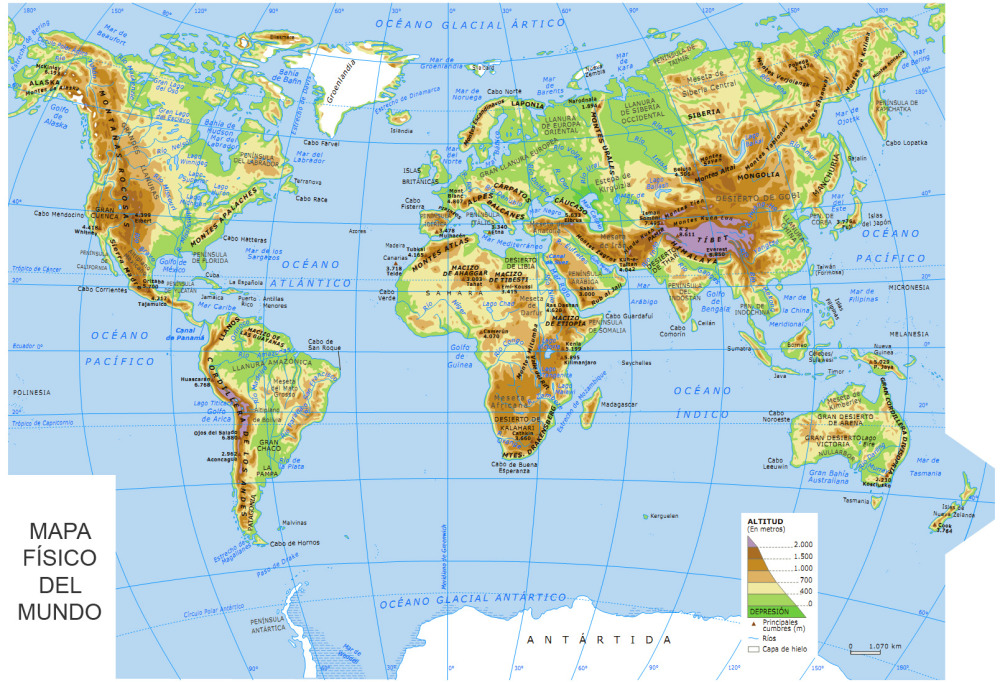
\includegraphics[width=\textwidth, frame, angle=90]{cuerpo/cap-objetos/imagenes/mapa-fisico}
	\caption[Figura rotada 1.]{Figura rotada 1. \textit{Método comando <<angle>>}: la imagen se rota 90\textdegree{} para aparecer apaisada, pero la página y el pie de página no. El tamaño se ha ajustado al ancho de linea.}
	\label{fig:mapa-fisico-a1}
\end{figure}
%\newpage
\lstinputlisting[frame={single}, language={[AlLaTeX]TeX}, label={cod-fig:mapa-fisico-a1}, caption=Código de la figura \ref{fig:mapa-fisico-a1}.]{cuerpo/cap-objetos/codigos/apaisado1.txt}
%
\begin{figure}[H]
	\centering
	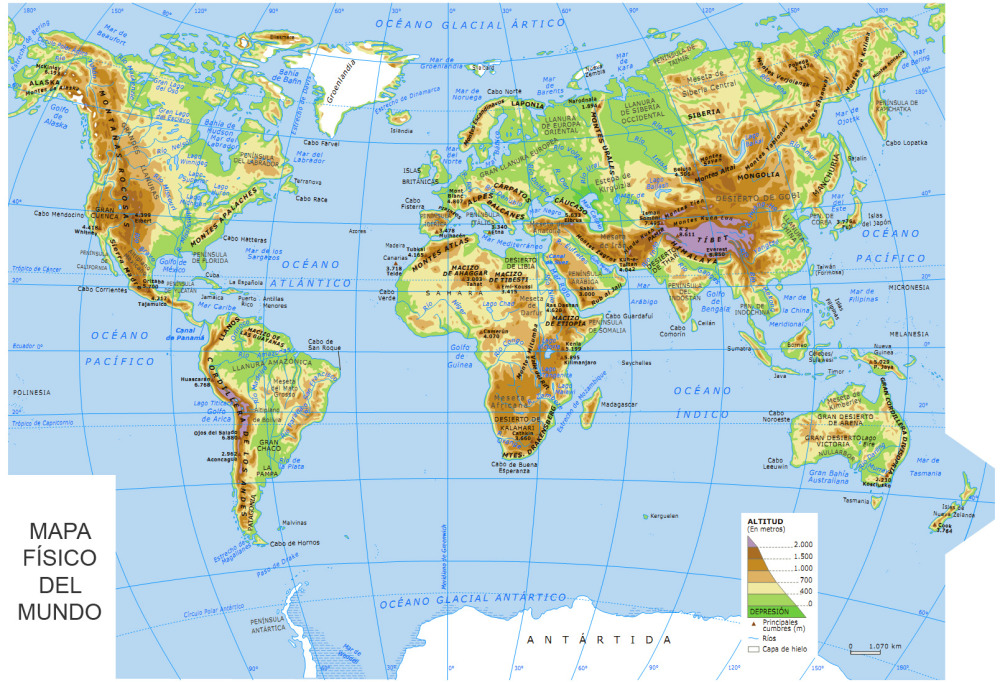
\includegraphics[scale=.65, frame, angle=90]{cuerpo/cap-objetos/imagenes/mapa-fisico}
	\caption[Figura rotada 2.]{Figura rotada 2.  \textit{Método comando <<angle>>}: la imagen se rota 90\textdegree{} para aparecer apaisada, pero la página y el pie de página no. El tamaño se ha ajustado a un 65\% del tamaño original.}
	\label{fig:mapa-fisico-a2}
\end{figure}
\newpage
\lstinputlisting[frame={single}, language={[AlLaTeX]TeX}, label={cod-fig:mapa-fisico-a2}, caption=Código de la figura \ref{fig:mapa-fisico-a2}.]{cuerpo/cap-objetos/codigos/apaisado2.txt}
%
\begin{sidewaysfigure}
	\centering
	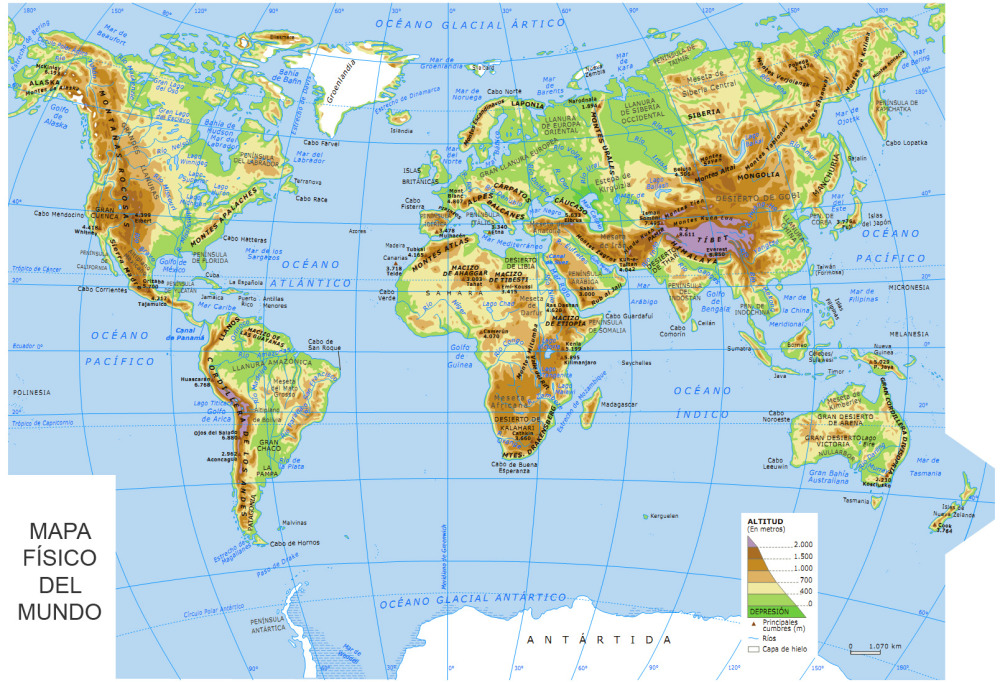
\includegraphics[width=\textwidth, frame]{cuerpo/cap-objetos/imagenes/mapa-fisico}
	\caption[Figura rotada 3.]{Figura rotada 3. \textit{Método entorno <<sidewaysfigure>>}: la imagen se rota automáticamente para aparecer apaisada, junto con el pie de página, pero la página en sí no. El tamaño se ha ajustado al ancho de linea.}
	\label{fig:mapa-fisico-a3}
\end{sidewaysfigure}
\lstinputlisting[frame={single}, language={[AlLaTeX]TeX}, label={cod-fig:mapa-fisico-a3}, caption=Código de la figura \ref{fig:mapa-fisico-a3}.]{cuerpo/cap-objetos/codigos/apaisado3.txt}
%
\begin{landscape}
	\begin{figure}[h]
		\centering
		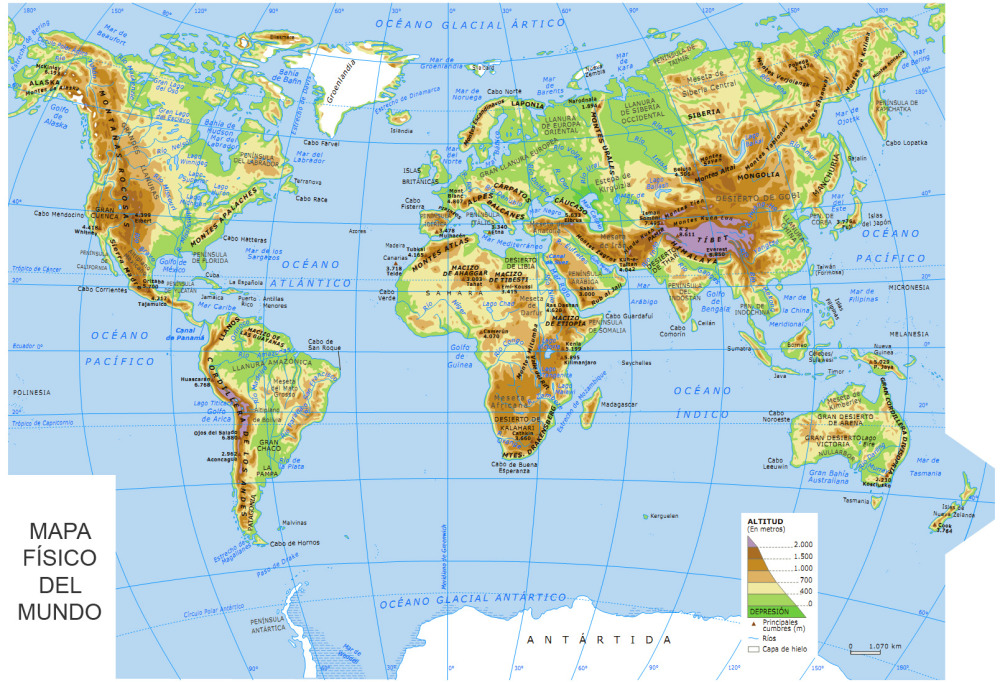
\includegraphics[scale=.65, frame, angle=0]{cuerpo/cap-objetos/imagenes/mapa-fisico}
		\caption[Figura rotada 4.]{Figura rotada 4. \textit{Método entorno <<landscape>>}: la página se rota automáticamente para aparecer apaisada incluido el pie de página, pero los encabezados no. El tamaño se ha ajustado a un 65\% del tamaño original. \hlc[green]{Método aconsejado}.}
		\label{fig:mapa-fisico-a4}
	\end{figure}
\end{landscape}
\lstinputlisting[language={[AlLaTeX]TeX}, label={cod-fig:mapa-fisico-a4}, caption=Código de la figura \ref{fig:mapa-fisico-a4}.]{cuerpo/cap-objetos/codigos/apaisado4.txt}
%
\begin{landscape}
	\begin{figure}
		\centering
		\begin{subfigure}[t]{.5\textwidth}
			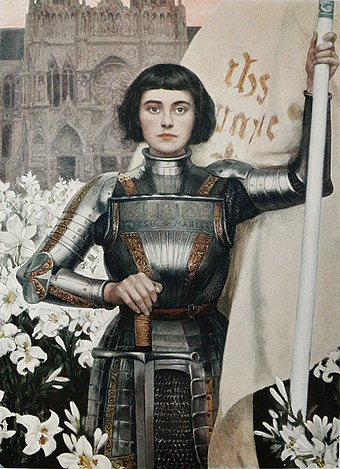
\includegraphics[width=\textwidth, frame]{cuerpo/cap-objetos/imagenes/juana-arco}
			\caption[Jean d´Arc]{Jean d´Arc. Grabado de Albert Lynch. Fuente: \cite{wikipedia-juana}.}
			\label{fig:juana-arco}
		\end{subfigure}
	%
		\begin{subfigure}[t]{0.5\textwidth}
			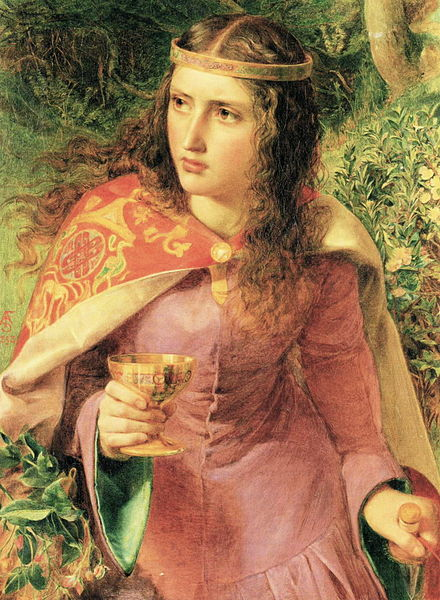
\includegraphics[width=\textwidth, frame]{cuerpo/cap-objetos/imagenes/eleanor-aquitania}
			\caption[Eleanor de Aquitania.]{Eleanor de Aquitania. Pintura de Frederick Sandys. Fuente: \cite{wikipedia-eleanor}.}
			\label{fig:eleanor-aquitania}
		\end{subfigure}
	\caption[Subfiguras en modo apaisado.]{Subfiguras en modo apaisado. Mujeres francesas del medievo.}
	\label{fig:subfiguras-apaisadas}
	\end{figure}
\end{landscape}
\lstinputlisting[frame={single}, language={[AlLaTeX]TeX}, label={cod-fig:subfiguras-apaisadas}, caption=Código de la figura \ref{fig:subfiguras-apaisadas}.]{cuerpo/cap-objetos/codigos/apaisado5.txt}
%
\chapter{Tablas}
3 opciones:
\begin{enumerate}
	\item Programar la tabla directamente; crear tablas en \LaTeX es complejo, no recomendado.
	\item Emplear una aplicación externa para crear la tabla en código \LaTeX e importarla al código; recomendaciones:
		\begin{itemize}
			\item  \href{https://www.tablesgenerator.com/}{https://www.tablesgenerator.com/}
			\item \href{https://www.latex-tables.com/}{https://www.latex-tables.com/}
		\end{itemize}
	\item Crear la imagen en un programa externo (hoja de cálculo, procesador de text, etc.) e incluirla como una imagen dentro de un entorno de tabla.
\end{enumerate}
%
\begin{table}[H]
	\centering
	\begin{tabular}{@{}lll@{}}
		\toprule
		Variable & Valor & Unidad \\ \midrule
		X        & 20    & N      \\
		Y        & 100   & kg     \\
		Z        & 0     & cm     \\ \bottomrule
	\end{tabular}
	\caption[Tabla creada con \url{https://www.tablesgenerator.com/}.]{Tabla creada con \url{https://www.tablesgenerator.com/}. Copiada directamente al \LaTeX.}
	\label{tab:tabla-1}
\end{table}
%
%tab:tabla-2
\begin{table}[H]
	\centering
	\begin{tabular}{@{}lll@{}}
		\toprule
		Variable & Valor & Unidad \\ \midrule
		A        & 0    & N      \\
		B        & 100   & kg     \\
		C        & 20     & cm     \\ \bottomrule
	\end{tabular}
	\caption[Tabla creada con \url{https://www.tablesgenerator.com/} bis]{Tabla creada con \url{https://www.tablesgenerator.com/} bis. El código se pega en un .tex específico y se importa al \LaTeX.}
	\label{tab:tabla-2}
\end{table}
%
\begin{table}[H]
	\centering
	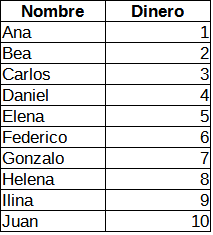
\includegraphics[scale=1]{cuerpo/cap-objetos/tablas/tabla-imagen-calc}
	\caption{Tabla desde una imagen.}
	\label{tab:tabla-3}
\end{table}

\begin{table}[H]
	\centering
	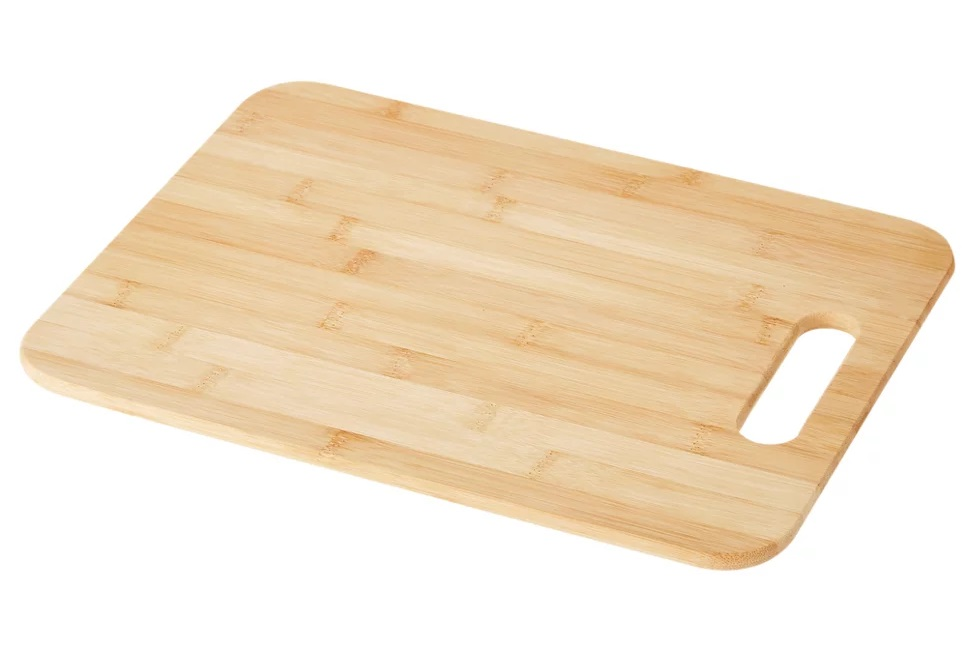
\includegraphics[width=1\textwidth, frame]{cuerpo/cap-objetos/tablas/tablas}
	\caption[Tabla desde una imagen bis.]{Tabla desde una imagen bis. Esta imagen es tratada como una tabla, apareciendo en el índice de tablas, y contando como tal par las referencias. La diferencia entre los entornos 'table' y 'figure' es puramente de distinción de items.}
	\label{tab:tabla-4}
\end{table}
\newpage
El código empleado es el mostrado en el fragmento \ref{cod-tablas}.
\lstinputlisting[frame={single}, language={[AlLaTeX]TeX}, label={cod-tablas}, caption=Código empleado para las tablas \ref{tab:tabla-1} a \ref{tab:tabla-2}.]{cuerpo/cap-objetos/codigos/tablas.txt}
%
\chapter{Documentos .pdf}
Los pdf se incluyen con el paquete \textit{pdfpages}, y su comando:
\lstinputlisting[language ={[AlLaTeX]TeX} , label ={cod-pdf} , caption ={
	Comando para incluir un documento .pdf. } , frame ={ single } , float ]{cuerpo/cap-objetos/codigos/include-pdf.txt}

\chapter{Planos}
%El sistema implementado en la plantilla está diseñado bajo 2 premisas:
\begin{enumerate}
	\item Los planos origen serán archivos .pdf.
	\item Los planos se agrupan por conjuntos, siendo estos los que aparecen en el índice de contenidos; y se crea índice de planos específico.
\end{enumerate}

Comandos y sintaxis:
\begin{enumerate}
	\item Crear e imprimir el índice de planos; estos comandos se deben insertar donde se quiera que aparezca el índice de planos.
	\lstinputlisting[frame={single}, language={[AlLaTeX]TeX}, label={cod-planos1}, caption=Comandos para el índice de planos]{cuerpo/cap-objetos/codigos/planos1.txt}
	%
	\item Invocar una nueva entrada en el índice de planos para separar conjuntos de planos.
	\lstinputlisting[frame={single}, language={[AlLaTeX]TeX}, label={cod-planos2}, caption=Comandos para crear un conjunto de planos que quedarán agrupados bajo una misma sección. Es esta etiqueta la que aparecerá en el índice de planos.]{cuerpo/cap-objetos/codigos/planos2.txt}
	\item Invocar una nueva entrada de plano.
	\lstinputlisting[frame={single}, language={[AlLaTeX]TeX}, label={cod-planos3}, caption=Comandos para invocar e incluir un nuevo plano.]{cuerpo/cap-objetos/codigos/planos1.txt}
\end{enumerate}
Se ha creado una macro para generar los pasos 2 y 3, disponible en el menú <<Macros>> del perfil, de nombre <<Add blueprint>>.
%
\chapter{Código}
Se puede incluir código de forma que sea tratado como un objeto, para crear un índice y usar referencias, e incluso resaltar palabras clave del lenguaje.

El método recomendado es mediante el paquete \href{https://www.ctan.org/pkg/listings}{\textit{listings}}. Se ha creado la macro <<Include code>> (y su botón correspondiente) en el perfil de TeXstudio para importar código desde archivos externos, que inserta el comando del fragmento \ref{cod-codigo-comando}:
\lstinputlisting[frame={single}, language={[AlLaTeX]TeX}, label={cod-codigo-comando}, caption=Linea insertada por la macro <<Include code>>.]{cuerpo/cap-objetos/codigos/codigo-comando.txt}

Se puede personalizar al cargar el paquete, en el archivo \textit{.../02-paquetes.tex} (colores, fuente, etc.).
%
\chapter{Expresiones matemáticas}
Las expresiones matemáticas son parte del código \LaTeX{} del documento, que se teclean directamente en el .tex, y dentro del modo matemático o en el entorno \textit{equation}. Cambian la tipografía a la matemática y activan comandos específicos para símbolos demás.
%
\section{Entorno matemático}\label{sec:entorno-matematico}
O \textit{math environment} o \textit{math mode}; su comportamiento por defecto es <<en linea>>, lo que permite alternarlo con modo texto; se activa encerrando la expresión deseada entre los símbolos \$\$.

Por ejemplo, si esto es un párrafo en el cual queremos integrar una expresión matemática como $ y = mb + c$, de forma que quede en linea con el resto del texto.
\lstinputlisting[frame={single}, language={[AlLaTeX]TeX}, label={cod-entorno-mat}, caption=Código del párrafo \ref{sec:entorno-matematico}.]{cuerpo/cap-objetos/codigos/mates-entorno-mat.txt}
%
\section{Entorno ecuación}
\textit{equation environment}, es un entorno de \LaTeX{} que imprime expresiones, por defecto, en una línea aparte, centrada, y opcionalmente con etiqueta para numerar. Se puede acceder mediante los botones mostrados en la figura \ref{fig:toolbar-lat}.

En este párrafo ponemos unos ejemplos; lorem ipsum lorem ipsum lorem ipsum; y aquí queremos una expresión matemática numerada:
\begin{equation}\label{ec-2-ley-newton}
	\sum \vec{F} = m \cdot \vec{a}
\end{equation}
Otro ejemplo más:
\begin{equation}\label{ec-einstein}
	e = mc^{2}
\end{equation}

Y para que no lleven etiqueta de numeración:
\begin{equation*}\label{ec-ley-ohm}
	V = I \cdot R
\end{equation*}
\lstinputlisting[frame={single}, language={[LaTeX]TeX}, label={cod-ecs}, caption=Código para expresiones matemáticas]{cuerpo/cap-objetos/codigos/mates-entorno-ecs.txt}
%
\chapter{Enumeraciones}
%
\begin{figure}[H]
	\centering
	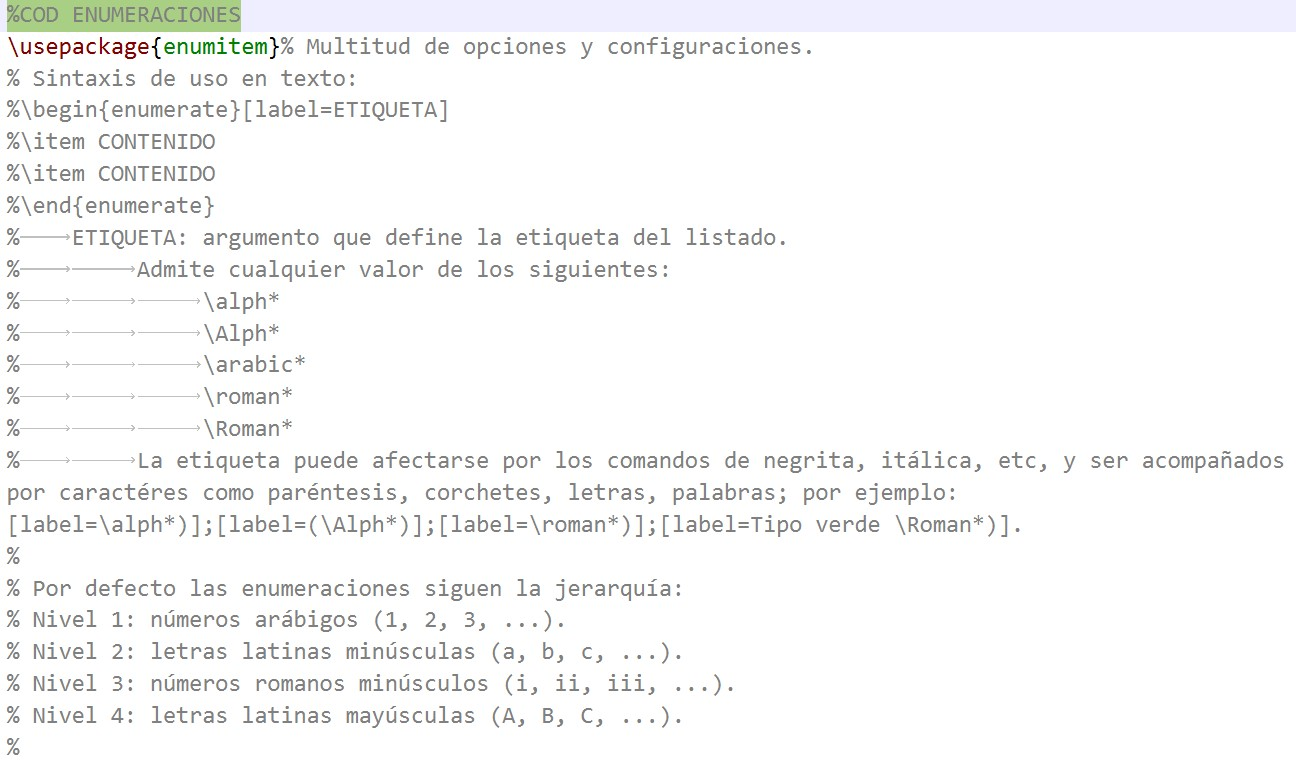
\includegraphics[width=1\linewidth, frame]{cuerpo/cap-objetos/imagenes/enumeraciones}
	\caption[Configuración de las enumeraciones.]{Configuración de las enumeraciones. Sintaxis para personalizar las enumeracions. Archivo: .../02-paquetes.tex.}
	\label{fig:enumeraciones}
\end{figure}
%
%
\begin{itemize}
\item\textbf{Enumeración por defecto:}
	\begin{enumerate}
		\item Elemento.
		\item Elemento.
		\item Elemento.
		\item Elemento.
		\item Elemento.
		\item Elemento.
		\item Elemento.
		\item Elemento.
	\end{enumerate}
%
\item\textbf{Enumeración por defecto en varias columnas:}
	\begin{multicols}{3}
		\begin{enumerate}
		\item Elemento.
		\item Elemento.
		\item Elemento.
		\item Elemento.
		\item Elemento.
		\item Elemento.
		\item Elemento.
		\item Elemento.
	\end{enumerate}
\end{multicols}
%
\item\textbf{Enumeración personalizada para usar letras minúsculas con paréntesis de cierre:}
	\begin{enumerate}[label=\alph*)]
		\item Elemento.
		\item Elemento.
		\item Elemento.
		\item Elemento.
	\end{enumerate}
%
\item\textbf{Enumeración personalizada para usar numeral romano precedido de la palabra <<caca>>:}
	\begin{enumerate}[label=caca \Roman*]
		\item Elemento.
		\item Elemento.
		\item Elemento.
		\item Elemento.
	\end{enumerate}
\end{itemize}
%
\chapter{Hiperenlaces}
Los hiperenlaces se incluyen mediante el paquete \textit{hyperref}; mediante el comando:
\begin{center}
	\textbackslash href \{URL\}\{TEXTO\}
\end{center}

Por ejemplo \href{https://en.wikipedia.org}{este enlace lleva a Wikipedia.}